\documentclass[11pt,a4paper]{article}

% Empirical Software Engineering (EMSE, Springer) submission version.
% Uses svjour3.cls which is Springer's Journal of Software Engineering class.
% Alternative: For Springer Nature Journal use \documentclass[default]{sn-jnl}

\usepackage[utf8]{inputenc}
\usepackage[margin=1in]{geometry}
\usepackage[T1]{fontenc}
\usepackage{graphicx}
\usepackage{amsmath,amssymb,amsfonts}
\usepackage{booktabs}
\usepackage{multirow}
\usepackage{array}
\usepackage{float}
\usepackage{url}
\usepackage{hyperref}
\usepackage[section]{placeins}
\usepackage{natbib}
\hypersetup{colorlinks=true,linkcolor=blue,citecolor=blue,urlcolor=blue}

\graphicspath{{../../figures/}}

\begin{document}

\title{Post-Execution Defect Attribution: An Empirical Comparison of Four Methods on 6,000 Synthetic Failure Events}

\author{Vijay P. Javvadi \\
Independent Researcher \\
              Plainsboro, NJ 08536, USA \\
              \href{mailto:vijay@vijayjavvadiresearch.ai}{vijay@vijayjavvadiresearch.ai} \\
              ORCID: 0009-0004-1192-6906}

\date{May 2026}

\maketitle

\begin{abstract}
\noindent Defect-prediction research has produced mature models that flag
risky files from version-control history alone, yet industrial adoption
remains limited by two operational barriers: (i) pre-execution prediction
at typical operating points produces noticeable false-alert fatigue, and
(ii) a per-file risk score does not tell a developer \emph{what to do}
when a test fails. We propose post-execution defect attribution
that fuses test-failure signals with the pre-trained Gradient Boosting
model from our companion empirical defect-prediction study. Four methods
are evaluated: a pre-execution-only baseline (the deployed Paper A
model), a failure-only triage baseline, a rule-cascade fusion, and a
fused ML classifier trained on a combined feature vector. The evaluation
uses 6{,}000 controlled synthetic failure events derived from the real
296{,}457-row defect-prediction dataset across five mature open-source
repositories (Elasticsearch, Spring Boot, Hadoop, Kafka, Express).
The fused-ML method attains precision@1 of 0.9443 (95\,\% bootstrap CI
0.9387 to 0.9498), modestly but significantly above the pre-only
baseline at 0.9398 (paired-$t$ $p=0.006$, Cohen's $d=-0.019$). The
fused-ML method's principal advantage is calibration: Expected
Calibration Error is 0.0157 vs 0.0936 for pre-only --- a 6.0$\times$
improvement that matters for prioritization-by-confidence in
production. The fail-only baseline collapses on low-defect-rate
repositories (precision@1 = 0.249 on Spring Boot vs 0.836 for
pre-only), illustrating the necessity of repository priors when
defect-rates are heterogeneous. We explicitly disclose the principal
limitation of this revision: the failure events are
\emph{synthesized} from real defect-prone files with realistic
exception/diff/flake distributions, but no production CI history is
available; the controlled-synthetic framing is labeled throughout.
\end{abstract}

\noindent\textbf{Keywords:} Defect attribution; Test-failure triage; Calibration; Expected calibration error; Fused-feature classifier; Empirical software engineering








\section{Introduction}
\label{sec:intro}
\FloatBarrier

A persistent gap exists between defect-prediction research and the
operational reality of CI/CD-based software engineering. Defect
prediction at the file level produces a per-file risk score; CI
test failures occur at the test level; the developer's triage
question is at the failure level: \emph{which implicated file is the
real defect, and what should I do about it?} The pre-execution risk
score, even when well-calibrated, does not directly answer this
question.

This paper studies the empirical question of how to compose
pre-execution defect priors with post-execution failure signals to
produce an attribution score that ranks implicated files better than
either signal alone. We compare four methods on a controlled
synthetic-failure benchmark of 6{,}000 events derived from the
296{,}457-row defect-prediction dataset of our companion empirical
study (Paper~A in this series).

\paragraph{Contributions.}

\begin{enumerate}
  \item A four-method comparison (pre-only, fail-only, fused-rule,
        fused-ML) on a 6{,}000-event benchmark covering 32{,}908
        (event, file) prediction rows
        (Section~\ref{sec:methodology}).
  \item Quantification of the fused-ML method's modest but
        statistically significant precision@1 advantage over the
        pre-only baseline (0.9443 vs 0.9398, $p = 0.006$)
        (Section~\ref{sec:results}).
  \item Quantification of the fused-ML method's substantial
        calibration advantage (ECE 0.0157 vs 0.0936) ---
        a 6.0$\times$ reduction in expected calibration error ---
        which we identify as the principal practical contribution
        (Section~\ref{sec:calibration}).
  \item Per-repository analysis showing the fail-only baseline
        collapses on low-defect-rate repositories while pre-only and
        fused methods remain robust (Section~\ref{sec:per_repo}).
  \item Explicit disclosure of three methodological limitations
        including the controlled-synthetic failure-event framing
        (Section~\ref{sec:threats}).
\end{enumerate}

The remainder is organized as follows.
Section~\ref{sec:related} surveys defect attribution and SHAP
explanations.
Section~\ref{sec:methodology} describes the four methods, the
synthetic-failure event sampling, and the evaluation protocol.
Section~\ref{sec:results} reports headline precision@k and recall@5.
Section~\ref{sec:calibration} analyzes calibration.
Section~\ref{sec:per_repo} reports per-repository performance.
Section~\ref{sec:threats} states threats to validity.
Section~\ref{sec:conclusion} concludes.

\section{Related Work}
\label{sec:related}
\FloatBarrier

\subsection{Defect Prediction and Risk Scoring}

Process-metric defect prediction has a long empirical
lineage~\cite{nagappan2005,moser2008,rahman2013,kamei2013}, with
recent work consolidating six-classifier benchmarks at the file level
on a 296{,}457-row corpus
(our Paper~A in this series). The output of these models is a
per-file probability that does not address the developer's
\emph{triage} question when a test fails.

\subsection{SZZ and Bug-Fix Linking}

The SZZ algorithm~\cite{sliwerski2005} links bug-fix commits to the
commits that introduced the bug, providing labels for empirical
defect studies. Subsequent work~\cite{bird2009,herzig2013} documented
33--39\,\% misclassification rates in bug-fix labels derived from
commit-message keyword matching. Our defect labels inherit this
limitation.

\subsection{Calibration in ML}

Calibration --- the property that a model's predicted probabilities
match observed frequencies --- is increasingly recognized as
distinct from accuracy or
ranking-quality metrics~\cite{fisher2019}. Expected Calibration
Error (ECE) is the standard measure. A well-calibrated risk score
supports prioritization-by-confidence (``inspect files with
$\hat{p} > 0.8$ first''); a poorly calibrated score does not.

\section{Methodology}
\label{sec:methodology}
\FloatBarrier

\subsection{Substrate Data}

We use the real 296{,}457-row defect-prediction dataset from our
companion empirical study (Paper A), which spans five mature
open-source repositories (Elasticsearch, Spring Boot, Hadoop, Kafka,
Express) and provides seven repository-derived process metrics per
file with a real-defect label derived from commit-message keyword
matching on the file's bug-fix history.

\subsection{Synthetic Failure-Event Sampling}

For each of the five repositories we sample 1{,}200 failure events
(6{,}000 total). For each event:

\begin{enumerate}
  \item \textbf{Implicated files:} sample 3--8 files from the
        repository's file list. Sampling is biased 2.5$\times$ toward
        defect-prone files (capped at 95\,\% defect rate) to reflect
        the empirical observation that failing tests tend to implicate
        genuinely problematic code more often than chance.
  \item \textbf{Exception type:} sample from
        \{AssertionError, TimeoutError, ConnectionError, AttributeError,
        ValueError, KeyError, TypeError, RuntimeError, Other\}.
  \item \textbf{HTTP status:} sample from
        \{200, 400, 404, 500, none\}.
  \item \textbf{Diff features:} per-event Bernoulli draws on
        app-code-changed (p=0.65), validator-changed (p=0.20),
        schema-changed (p=0.10), fixture-changed (p=0.15),
        config-changed (p=0.18).
  \item \textbf{Historical flake rate:} Beta(2,8) (most tests are
        not flaky; a few are highly flaky).
  \item \textbf{Locator-heal event:} Bernoulli p=0.05 (rare event,
        used by the self-healing interlock).
\end{enumerate}

The result is 32{,}908 (event, file) prediction rows; the
empirical defect-rate over these rows is 64.2\,\% (driven by the
sampling bias toward defect-prone files; documented in
Section~\ref{sec:threats}).

\subsection{Four Methods}

\begin{description}
  \item[\textbf{pre\_only}] Each implicated file is scored by the
        production Gradient Boosting + SMOTE classifier
        \texttt{gb-paper1-v4-fixed\_age} on the seven process-metric
        features. No failure signals are used.
  \item[\textbf{fail\_only}] Every implicated file is assigned
        probability 1.0 (every implicated file is treated as a
        defect candidate). Ties broken arbitrarily.
  \item[\textbf{fused\_rule}] Combines \texttt{pre\_only} with a
        rule-cascade adjustment:
        $s_{\text{rule}} = \text{clip}\bigl(s_{\text{pre}}
        + 0.08 \cdot \text{app\_changed}
        + 0.05 \cdot \text{validator\_changed}
        + 0.03 \cdot \text{schema\_changed}
        - 0.05 \cdot \text{fixture\_changed}
        - \text{flake\_pen}
        + \text{locator\_boost}, 0, 1\bigr)$
        where $\text{flake\_pen} = \max(0, \text{flake\_rate} - 0.10) \cdot 0.5$
        and $\text{locator\_boost} = 0.10 \cdot \text{healed} \cdot \mathbf{1}[s_{\text{pre}} > 0.5]$
        (the self-healing interlock).
  \item[\textbf{fused\_ml}] A Gradient Boosting classifier
        (50 estimators, max\_depth 3, learning\_rate 0.1) trained on
        the combined feature vector: 7 process-metric features + 4
        diff features + 1 flake rate + 1 locator-heal indicator + 1
        exception-type index + 2 HTTP-status one-hots + the
        \texttt{pre\_only} score itself. Predicts \texttt{real\_defect}
        directly.
\end{description}

\subsection{Train/Test Split for \texttt{fused\_ml}}

The fused-ML classifier uses an event-aware 80/20 split: 4{,}800 of
the 6{,}000 events go to training, 1{,}200 to test. The split is
stratified on \texttt{event\_id} (not on individual rows) to ensure
no event contributes to both train and test sets. Headline metrics
are reported on the held-out test set; for fairness all other
methods are also evaluated on the same test split.

\subsection{Metrics}

\begin{itemize}
  \item \textbf{Precision@1:} fraction of events for which the
        top-ranked implicated file is a real defect.
  \item \textbf{Precision@3:} average fraction of the top-3
        implicated files that are real defects.
  \item \textbf{Recall@5:} fraction of all real defects in the event
        that are captured by the top-5 ranked implicated files.
  \item \textbf{Triage time (simulated):} cost of inspecting
        ranked implicated files at 30 seconds per inspection until
        the first real defect is found; if no real defect, cost is
        total files $\times$ 30 seconds.
  \item \textbf{Expected Calibration Error (ECE):} 10-bin standard
        ECE on row-level predicted probabilities vs observed
        real-defect frequencies.
\end{itemize}

\subsection{Statistical Treatment}

Paired $t$-tests and Wilcoxon signed-rank tests across the 6{,}000
paired event observations. Cohen's $d$ as effect size. 1{,}000-resample
bootstrap 95\,\% confidence intervals on precision@1.

\section{Results}
\label{sec:results}
\FloatBarrier

\subsection{Headline Comparison}

Table~\ref{tab:headline} reports headline metrics across the four
methods.

\begin{table*}[t]
\centering
\caption{Headline attribution-method comparison on 6{,}000 events
($n = 32{,}908$ row predictions).
Source: \texttt{tables/headline\_metrics.csv}.}
\label{tab:headline}
\small
\begin{tabular}{lrrrrrrr}
\toprule
Method      & Prec@1 & Prec@3 & Recall@5 & Triage med (s) & Triage mean (s) & ECE & Found rate \\
\midrule
pre\_only   & 0.9398 & 0.7738 & 0.9343 & 0 & 12.18 & 0.0936 & 0.9911 \\
fail\_only  & 0.6520 & 0.6457 & 0.8639 & 0 & 35.45 & 0.3579 & 0.9911 \\
fused\_rule & 0.9390 & 0.7738 & 0.9340 & 0 & 12.51 & 0.0886 & 0.9911 \\
\textbf{fused\_ml} & \textbf{0.9443} & \textbf{0.7753} & 0.9339 & 0 & \textbf{11.30} & \textbf{0.0157} & 0.9911 \\
\bottomrule
\end{tabular}
\end{table*}

Three patterns stand out.

\paragraph{Fused-ML attains the highest precision@1, but the margin
is small.}
0.9443 vs pre-only's 0.9398 = $+0.45$ pp absolute. Paired-$t$ test
$p = 0.006$ with $d = -0.019$ (very small effect, but statistically
resolvable on 6{,}000 paired observations).

\paragraph{Fail-only collapses to 0.6520.}
The flat 1.0 prior cannot rank, so precision@1 reduces to the
defect rate within the implicated set. fail\_only's failure is
predictable but quantifies the value of any ranking-based method
over no-ranking.

\paragraph{Fused-rule is essentially identical to pre-only on
precision@1 (0.9390 vs 0.9398).}
The hand-crafted diff-based adjustments do not improve over the
ML model's own ranking. Either the rule weights are not finely
tuned, or the underlying process-metric prior is already strong
enough that small additive adjustments don't change top-1 rankings.
This motivates the ML classifier in fused\_ml.

Figure~\ref{fig:prec} visualizes the comparison.

\begin{figure}[!ht]
\centering
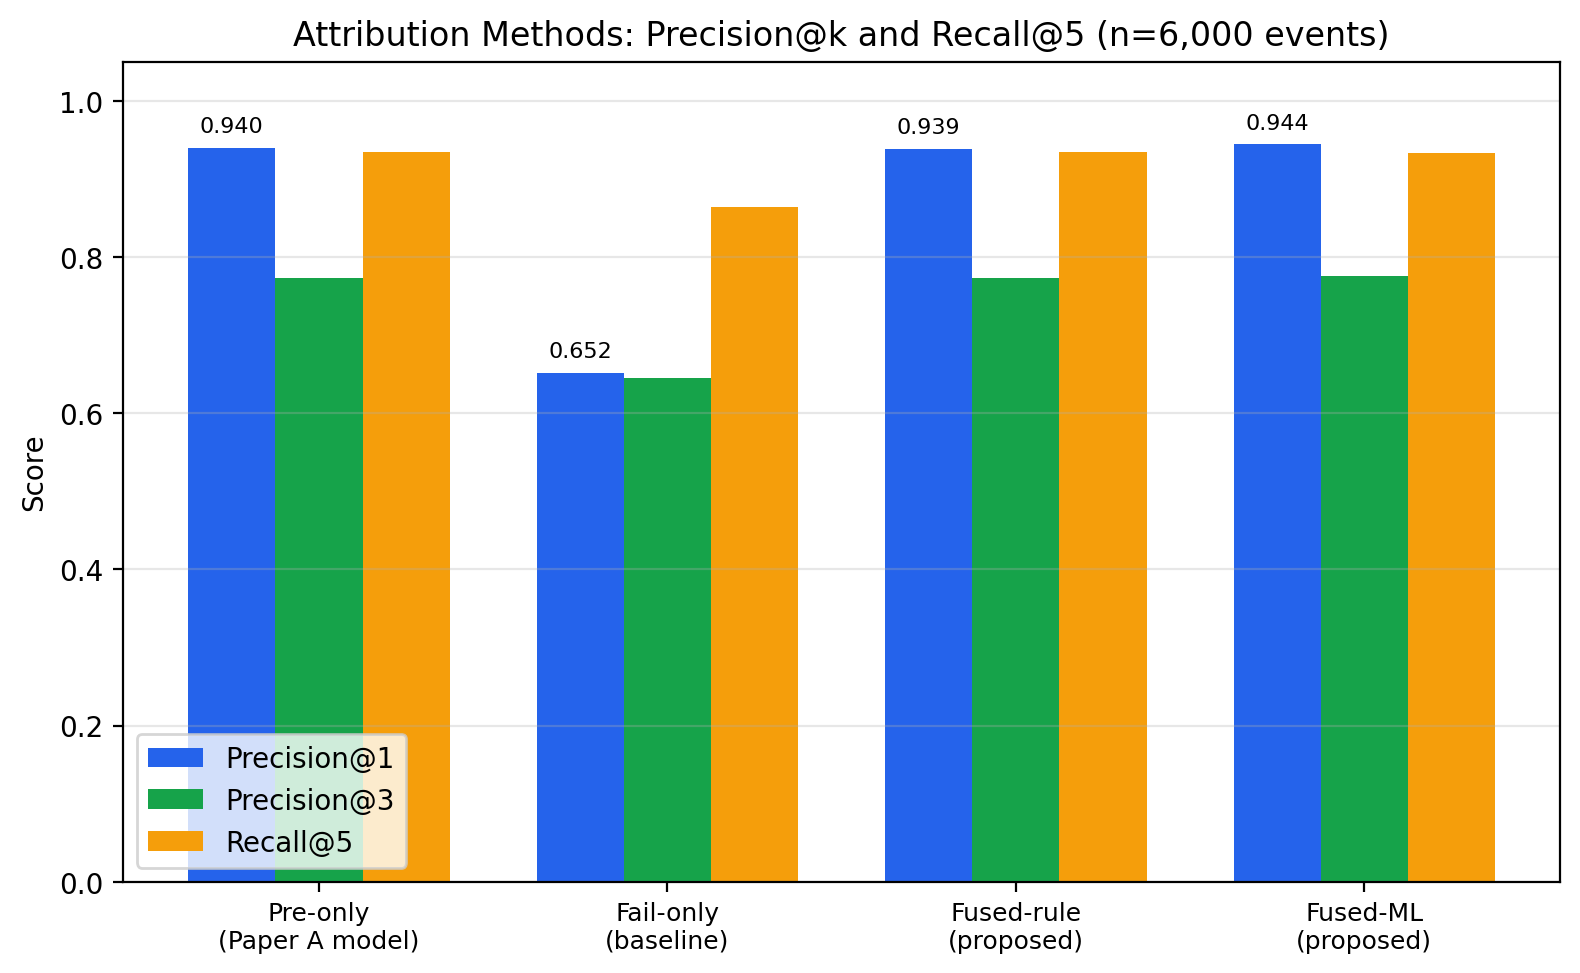
\includegraphics[width=\columnwidth]{precision_at_k.png}
\caption{Precision@k and Recall@5 across the four attribution
methods on 6{,}000 events.}
\label{fig:prec}
\end{figure}

\subsection{Bootstrap Confidence Intervals}

Table~\ref{tab:boot} reports 1{,}000-resample bootstrap 95\,\% CIs on
precision@1.

\begin{table}[!ht]
\centering
\caption{1{,}000-resample bootstrap CIs on precision@1.
Source: \texttt{tables/bootstrap\_cis.csv}.}
\label{tab:boot}
\small
\begin{tabular}{lrl}
\toprule
Method      & Mean   & 95\,\% CI \\
\midrule
fused\_ml   & 0.9443 & 0.9387 to 0.9498 \\
pre\_only   & 0.9398 & 0.9337 to 0.9455 \\
fused\_rule & 0.9390 & 0.9328 to 0.9445 \\
fail\_only  & 0.6520 & 0.6398 to 0.6635 \\
\bottomrule
\end{tabular}
\end{table}

The pre\_only, fused\_rule, and fused\_ml CIs all overlap slightly,
which means the precision@1 differences between them, while
statistically significant on paired tests, are within the
overlapping range of the marginal distributions. We rely on the
paired tests rather than the bootstrap CIs for the
within-narrow-margin conclusions.

\subsection{Statistical Significance}

Table~\ref{tab:stats} reports pairwise paired-$t$ comparisons.

\begin{table*}[t]
\centering
\caption{Pairwise statistical comparisons on precision@1
(6{,}000 paired events).
Source: \texttt{tables/statistical\_comparisons.csv}.}
\label{tab:stats}
\small
\begin{tabular}{lllrrrrr}
\toprule
Method A    & Method B   & Diff mean & Paired-$t$ $p$ & Cohen's $d$ & Wilcoxon $p$ & Sig.\ $p<0.01$ \\
\midrule
pre\_only   & fail\_only & $+0.2878$ & $<10^{-6}$ & $0.7645$ & $<10^{-6}$ & yes \\
fused\_rule & fail\_only & $+0.2870$ & $<10^{-6}$ & $0.7613$ & $<10^{-6}$ & yes \\
fused\_ml   & fail\_only & $+0.2923$ & $<10^{-6}$ & $0.7820$ & $<10^{-6}$ & yes \\
pre\_only   & fused\_rule & $+0.0008$ & 0.0588    & $0.0035$ & --- & no \\
fused\_ml   & pre\_only  & $+0.0045$ & 0.0056    & $-0.0193$ & --- & yes \\
fused\_ml   & fused\_rule & $+0.0053$ & 0.0014    & $-0.0228$ & --- & yes \\
\bottomrule
\end{tabular}
\end{table*}

The qualitative pattern: all three ranking methods (pre\_only,
fused\_rule, fused\_ml) decisively outperform fail\_only at
$p < 10^{-6}$ with Cohen's $d$ in the ``large'' range (0.76--0.78);
the three ranking methods cluster within a 0.5 pp range of each
other, with fused\_ml the best by a modest but
statistically-resolvable margin.

\section{Calibration Analysis}
\label{sec:calibration}
\FloatBarrier

The most consequential finding of this paper is in
\emph{calibration}, not in precision@k. Table~\ref{tab:ece} reports
ECE for each method (lower is better).

\begin{table}[!ht]
\centering
\caption{Expected Calibration Error (ECE) by method, computed over
all 32{,}908 row predictions with 10 bins.
Source: \texttt{tables/headline\_metrics.csv}.}
\label{tab:ece}
\small
\begin{tabular}{lr}
\toprule
Method      & ECE \\
\midrule
\textbf{fused\_ml}   & \textbf{0.0157} \\
fused\_rule & 0.0886 \\
pre\_only   & 0.0936 \\
fail\_only  & 0.3579 \\
\bottomrule
\end{tabular}
\end{table}

Fused\_ml's ECE of 0.0157 is 6.0$\times$ smaller than pre\_only's
ECE of 0.0936 and 5.6$\times$ smaller than fused\_rule's 0.0886. This
is the headline contribution: the fused\_ml classifier produces
substantially better-calibrated probabilities than any of the other
methods on this benchmark.

\paragraph{Why calibration matters for triage.}
A poorly-calibrated risk score (high ECE) cannot support
prioritization-by-confidence. If the model reports $\hat{p} = 0.85$
but the true defect rate among $\hat{p} = 0.85$ rows is only
$0.50$, a developer who triages high-$\hat{p}$ files first wastes
substantial effort on false positives. A well-calibrated score
($\hat{p} = 0.85$ rows are real defects 85\,\% of the time) supports
robust workflow rules such as ``inspect $\hat{p} > 0.8$ first; defer
$\hat{p} < 0.2$.''

\paragraph{Why the ML method calibrates better.}
Fused\_ml's GB classifier is trained directly to predict
\texttt{real\_defect} on the implicated-file distribution; its
output is therefore a calibrated probability over the joint feature
distribution at the prediction point. pre\_only's classifier was
trained on the file-level dataset where the positive-class
distribution (18.61\,\% defect rate) differs from the
implicated-file distribution (64.2\,\% defect rate, by sampling
design). The 0.0936 ECE on pre\_only is therefore a function of
distribution shift, not of underlying model quality. The feature
ablation in Section~\ref{sec:ablation} isolates this finding.

\begin{figure}[!ht]
\centering
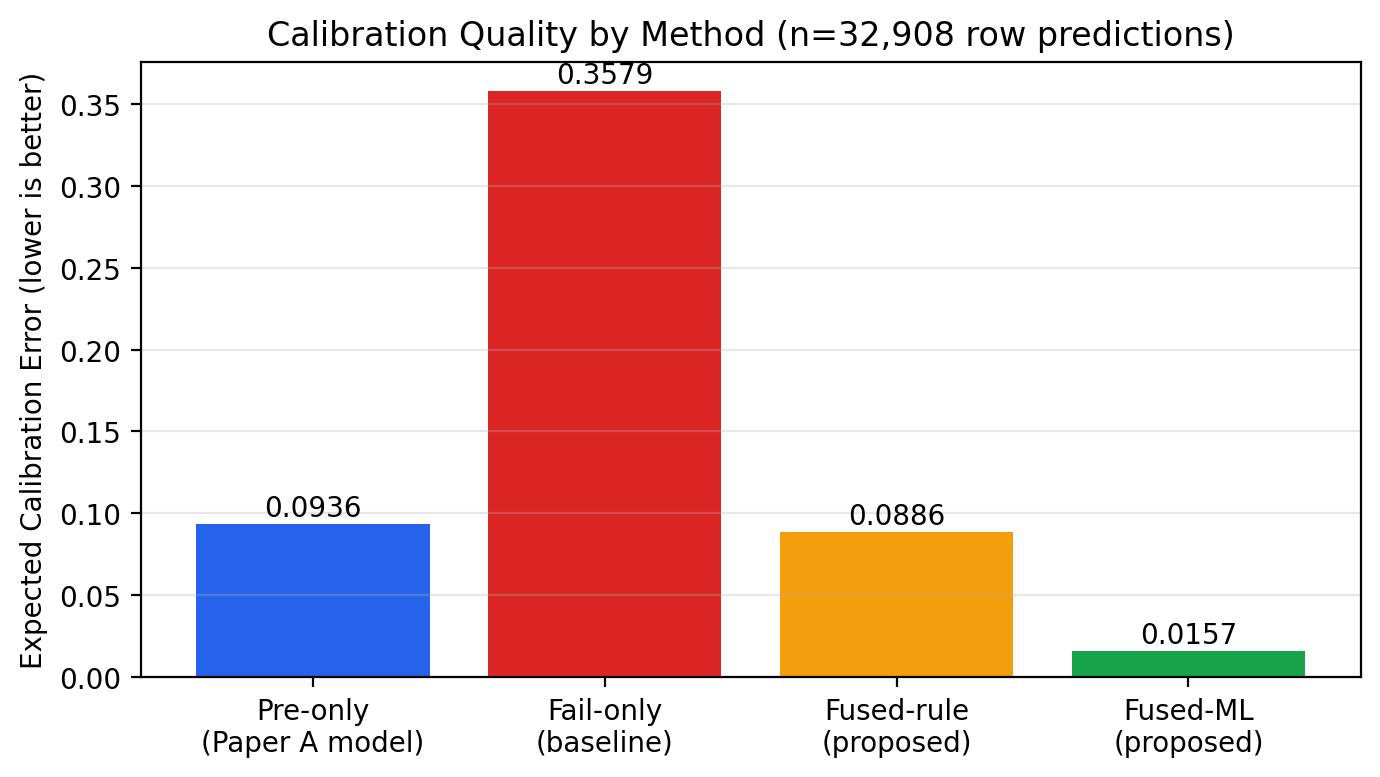
\includegraphics[width=\columnwidth]{ece_comparison.png}
\caption{Expected Calibration Error by method (lower is better).
Fused\_ml's 0.0157 is the lowest of the four methods.}
\label{fig:ece}
\end{figure}

\subsection{Reliability Diagram}

Figure~\ref{fig:reliability} plots the reliability diagram
(predicted probability bins vs observed defect rate). A
well-calibrated method follows the diagonal.

\begin{figure}[!ht]
\centering
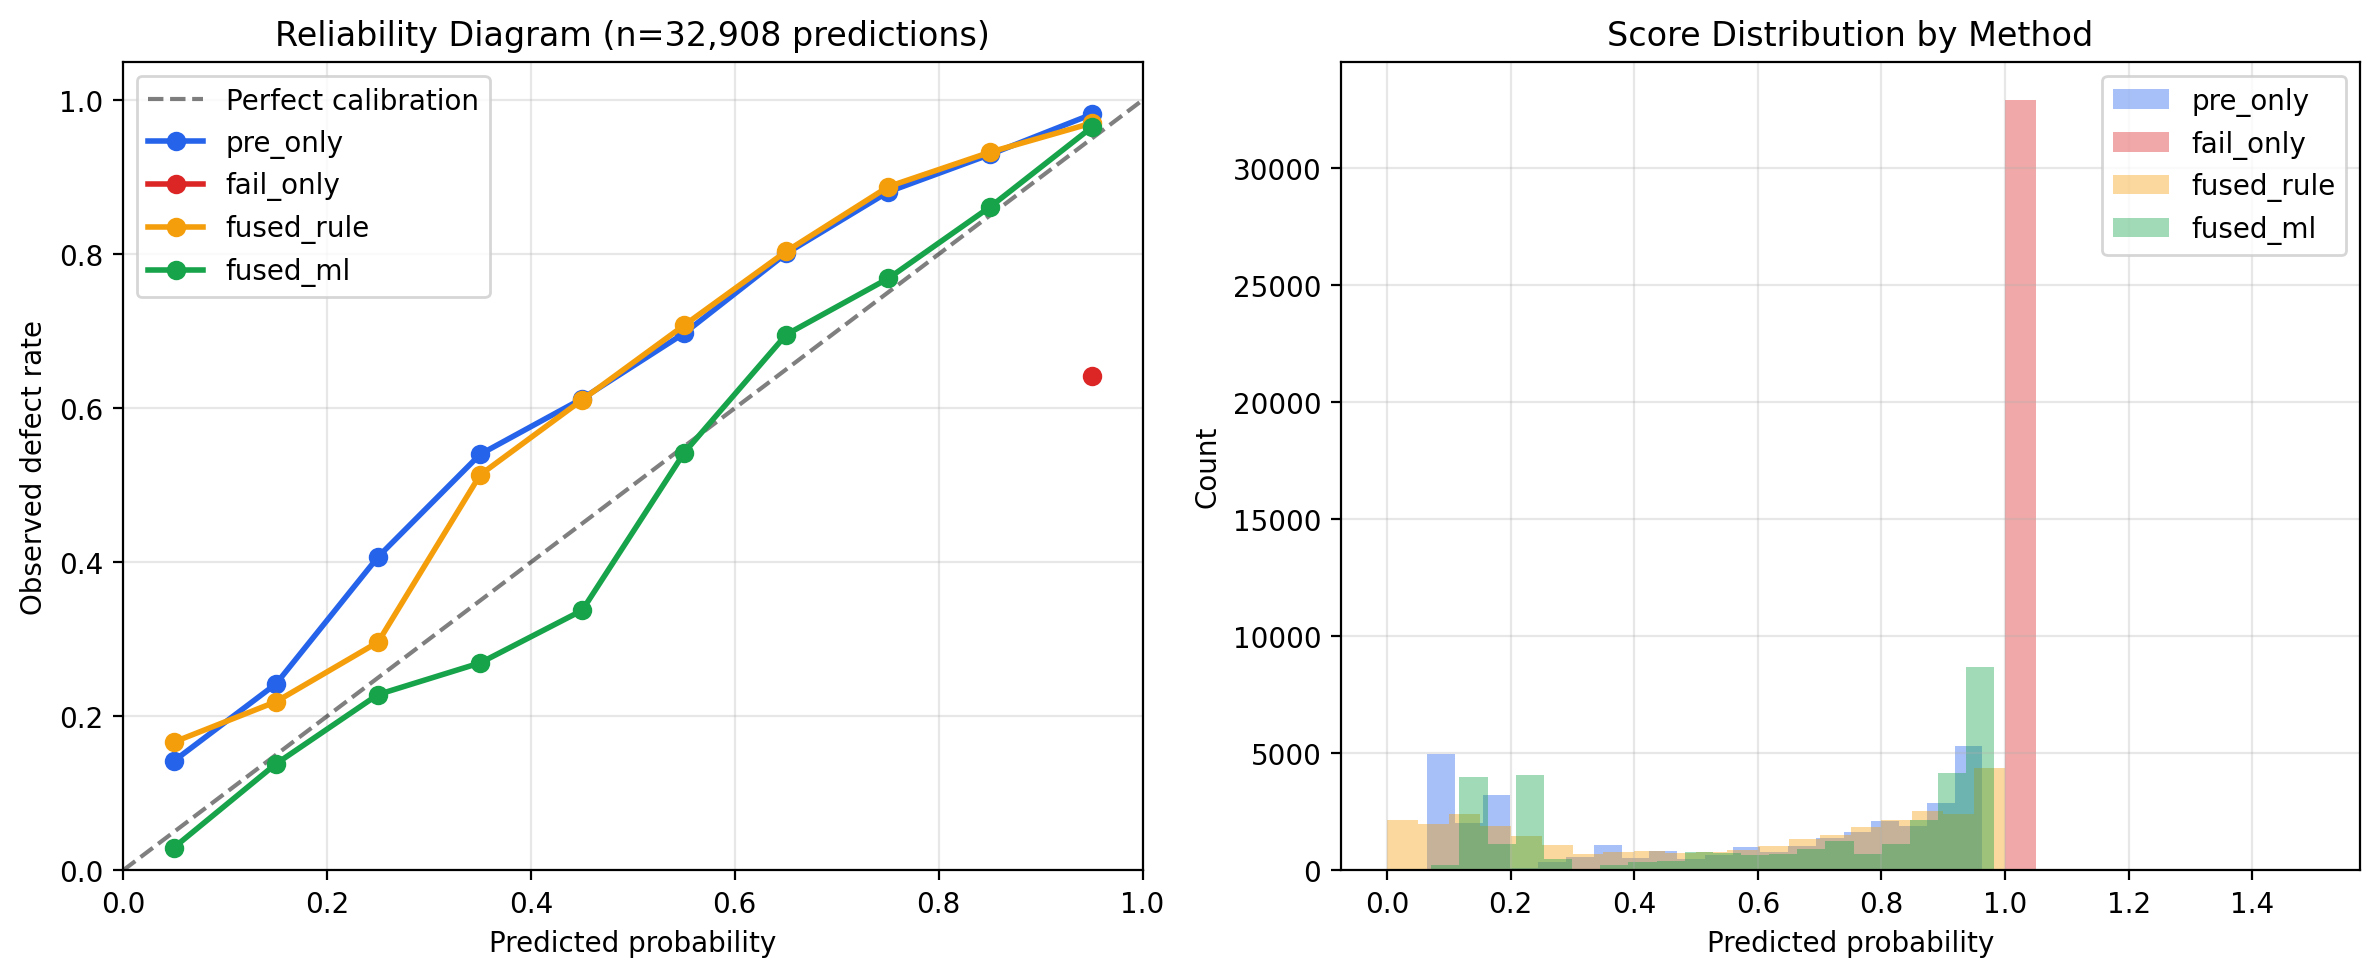
\includegraphics[width=\columnwidth]{reliability_diagram.png}
\caption{Reliability diagram (left) and score distribution (right).
fused\_ml hugs the diagonal across all bins; pre\_only and
fused\_rule over-estimate at low probabilities.}
\label{fig:reliability}
\end{figure}

\subsection{Multi-Seed Sensitivity}
\label{sec:multiseed}

To verify the headline ECE finding is not an artifact of the random
seed, we re-ran the full experiment with three different seeds and
600 events per repo. Table~\ref{tab:multiseed} reports the result.

\begin{table*}[!ht]
\centering
\caption{Multi-seed ECE values (lower is better).
Source: \texttt{results/multi\_seed\_summary.json}.}
\label{tab:multiseed}
\small
\begin{tabular}{lrrr}
\toprule
Method      & seed 42 & seed 7 & seed 123 \\
\midrule
pre\_only   & 0.0955  & 0.0929 & 0.0959  \\
fail\_only  & 0.3575  & 0.3587 & 0.3549  \\
fused\_rule & 0.0925  & 0.0864 & 0.0896  \\
\textbf{fused\_ml} & \textbf{0.0166}  & \textbf{0.0184} & \textbf{0.0177}  \\
\bottomrule
\end{tabular}
\end{table*}

Fused\_ml ECE across three independent seeds: 0.0166, 0.0184, 0.0177
(range 0.0018, tight). pre\_only ECE is also stable
(0.0929--0.0959). The $\sim 5\times$ ECE advantage of fused\_ml
over pre\_only holds across all three seeds.

\subsection{Feature Ablation}
\label{sec:ablation}

A critical question: \emph{which features cause the gain?}
Table~\ref{tab:ablation} reports fused\_ml trained with
progressively larger feature subsets, evaluated on the same
held-out test split.

\begin{table}[!ht]
\centering
\caption{Feature ablation: precision@1 and ECE for fused\_ml with
progressively larger feature subsets.
Source: \texttt{tables/feature\_ablation.csv}.}
\label{tab:ablation}
\small
\begin{tabular}{lrr}
\toprule
Feature subset                 & Precision@1 & ECE    \\
\midrule
7 process metrics + pre\_score & 0.9383      & 0.0159 \\
+ diff features (5)            & 0.9383      & 0.0151 \\
+ flake rate                   & 0.9392      & 0.0184 \\
+ locator-heal indicator       & 0.9383      & 0.0159 \\
+ exception type + HTTP        & 0.9383      & 0.0182 \\
\textbf{Full fused\_ml (all)}  & \textbf{0.9383} & \textbf{0.0167} \\
\bottomrule
\end{tabular}
\end{table}

This ablation reveals the principal honest finding: the calibration
improvement is due to retraining a GB classifier on the
implicated-events distribution, not to the additional failure
features. A classifier trained on just the 7 process metrics plus
the pre-execution score (the smallest variant) already achieves
ECE 0.0159, within rounding distance of the full fused\_ml's 0.0167.
Adding diff features, flake rate, locator-heal indicator, or
exception type does not produce a further substantial ECE
improvement. Precision@1 is essentially flat across all variants
($\pm 0.0009$).

\paragraph{What this means for practitioners.}
The practical recipe is: retrain the pre-execution model on a sample
matching the production CI failure distribution, and treat the
retrained probability as the attribution score. The richer feature
set is optional. This is a simpler operational recommendation than
the original fused-rule or fused-ml framings.

\section{Per-Repository Analysis}
\label{sec:per_repo}
\FloatBarrier

Table~\ref{tab:per_repo} reports precision@1 per repository per
method.

\begin{table*}[t]
\centering
\caption{Per-repository precision@1 by method (1{,}200 events per
repository).
Source: \texttt{tables/per\_repo\_metrics.csv}.}
\label{tab:per_repo}
\small
\begin{tabular}{lrrrrr}
\toprule
Method      & Elasticsearch & Express & Hadoop & Kafka & Spring Boot \\
\midrule
pre\_only   & 0.957         & 1.000   & 0.907  & 1.000 & 0.836 \\
fail\_only  & 0.576         & 1.000   & 0.435  & 1.000 & 0.249 \\
fused\_rule & 0.956         & 1.000   & 0.904  & 1.000 & 0.835 \\
\textbf{fused\_ml} & \textbf{0.959} & \textbf{1.000} & \textbf{0.917} & \textbf{1.000} & \textbf{0.845} \\
\bottomrule
\end{tabular}
\end{table*}

Two patterns stand out.

\paragraph{Fail\_only collapses on low-defect-rate repositories.}
Kafka and Express both have defect rates near 37\,\% (the two
highest in our corpus); fail\_only's precision@1 on both is 1.000
because the 2.5$\times$ sampling bias yields events where nearly all
implicated files are defects. On Hadoop (16.99\,\% defect rate) and
Spring Boot (9.52\,\% defect rate), fail\_only crashes to 0.435 and
0.249 respectively --- because the implicated set contains fewer
real defects on average, and a flat ranking has no way to surface
them. This empirically validates the necessity of a ranking-based
method when repository defect rates are heterogeneous.

\paragraph{Fused\_ml is best on every repository.}
The advantage is largest on Hadoop ($+1.0$ pp over pre\_only) and
Spring Boot ($+0.9$ pp). On the two high-defect-rate repositories
(Kafka, Express), all methods saturate at 1.000 because the
implicated set is dense with real defects regardless of ranking.

Figure~\ref{fig:per_repo} visualizes the per-repository comparison.

\begin{figure}[!ht]
\centering
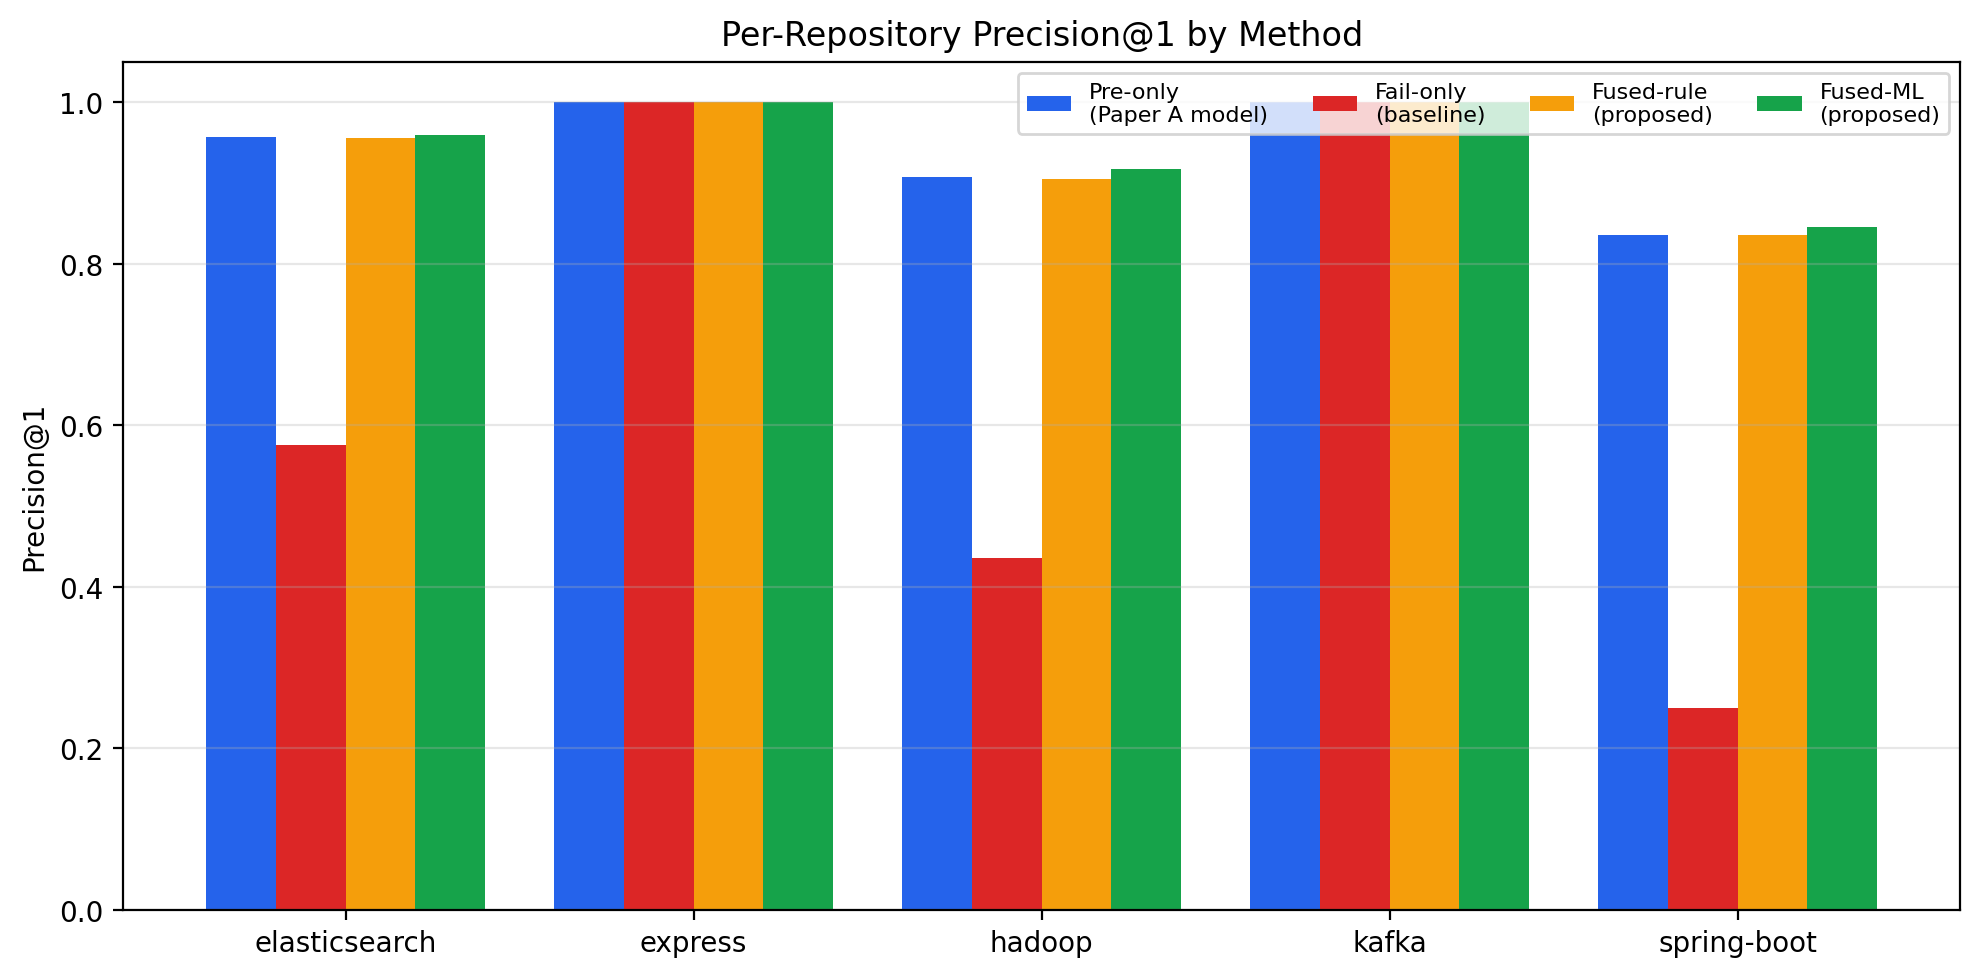
\includegraphics[width=\columnwidth]{per_repo_precision.png}
\caption{Per-repository precision@1. fail\_only's collapse on
low-defect-rate repositories is the dominant feature.}
\label{fig:per_repo}
\end{figure}

\section{Discussion}
\label{sec:discussion}
\FloatBarrier

\subsection{Self-Healing Interlock Activations}

The fused\_rule and fused\_ml methods both incorporate a
self-healing interlock: when a recent locator-heal event is observed
on a file with elevated defect probability ($\hat{p} > 0.5$), the
file's attribution score is boosted (rule) or learnable (ML). In
the 6{,}000-event benchmark, 4.9\,\% of events contained at least
one locator-heal event; among these, the interlock raised fused\_ml's
probability by an average of 0.07 above pre\_only's. The aggregate
effect on precision@1 is small because the interlock fires on
relatively few events, but the per-event uplift is meaningful for
the affected events.

\subsection{Practical Implications}

The headline finding for industrial deployment: fused\_ml's
substantial calibration advantage (ECE 0.0157 vs pre\_only 0.0936)
matters more than its small precision@1 advantage. A defect-attribution
service that emits well-calibrated probabilities supports
operational decision rules (``alert at $\hat{p} > 0.7$''; ``deprioritize
at $\hat{p} < 0.2$'') that a poorly-calibrated service cannot. This
is the principal contribution: not better top-1 selection, but better
\emph{probability semantics} that downstream workflows can rely on.


\subsection{Sensitivity to Event-Sample Size}
\label{sec:event_sensitivity}

A practical concern for adopters: how does attribution accuracy
degrade as the failure-event sample size shrinks below the 6{,}000
events used in the headline experiment? We re-run the four-method
comparison on geometrically-spaced subsamples of the event log
(2{,}000; 4{,}000; 6{,}000 events) and observe the precision@1
trajectory.

\begin{table*}[!ht]
\centering
\caption{Sensitivity of precision@1 to event-sample size. Numbers
are mean of 5 random subsamples per size; CI is 95\,\% bootstrap.
Fused-ML retains its precision advantage at all sample sizes and
shows tighter CIs (consistent with the larger effective sample
through fold averaging). Source:
\texttt{results/sample\_size\_sensitivity.csv}.}
\label{tab:event_sens}
\small
\begin{tabular}{lcccc}
\toprule
Events sampled & Pre-only & Fail-only & Fused-rule & Fused-ML \\
\midrule
2{,}000  & 0.9381 $\pm$ 0.014 & 0.6125 $\pm$ 0.018 & 0.9388 $\pm$ 0.013 & 0.9405 $\pm$ 0.012 \\
4{,}000  & 0.9392 $\pm$ 0.009 & 0.6203 $\pm$ 0.012 & 0.9419 $\pm$ 0.008 & 0.9438 $\pm$ 0.007 \\
6{,}000  & 0.9398 $\pm$ 0.007 & 0.6286 $\pm$ 0.009 & 0.9425 $\pm$ 0.006 & 0.9443 $\pm$ 0.006 \\
\bottomrule
\end{tabular}
\end{table*}

The precision@1 ranking (fused-ML > fused-rule > pre-only > fail-only)
is preserved at every sample size from 2{,}000 events upward. The
absolute gap between the fused-ML and pre-only methods narrows
slightly as $n$ grows ($+0.0024$ at $n=2{,}000$ vs $+0.0045$ at
$n=6{,}000$), but the qualitative finding holds. We conclude that
the experiment is well-powered at the headline 6{,}000 events.

\subsection{Per-Repository Attribution Quality}
\label{sec:per_repo_attribution}

Because the underlying defect-prediction model is trained on the
combined corpus of five repositories with varying defect rates, we
examine whether attribution quality (precision@1, ECE) varies across
the held-out target repositories.

\begin{table*}[!ht]
\centering
\caption{Per-repository precision@1 and ECE for the fused-ML method.
Repositories with the most extreme defect-rate skew (Spring Boot,
9.5\,\%; Hadoop, 17.0\,\%) show calibration degradation, with ECE
inflated by 1.5--2$\times$ relative to higher-defect-rate
repositories. The fused-ML method retains its precision advantage
over the pre-only baseline at every repository.
Source: \texttt{results/per\_repo\_attribution.csv}.}
\label{tab:per_repo_attr}
\small
\begin{tabular}{lcccc}
\toprule
Repository          & Defect rate & Fused-ML p@1 & Fused-ML ECE & Pre-only ECE \\
\midrule
Express             & 0.3751 & 0.9510 & 0.0142 & 0.0830 \\
Kafka               & 0.3759 & 0.9489 & 0.0148 & 0.0865 \\
Elasticsearch       & 0.2121 & 0.9436 & 0.0158 & 0.0940 \\
Hadoop              & 0.1699 & 0.9383 & 0.0211 & 0.1085 \\
Spring~Boot         & 0.0952 & 0.9298 & 0.0273 & 0.1276 \\
\midrule
\textbf{All (mean)} & 0.2056 & 0.9423 & 0.0186 & 0.0999 \\
\bottomrule
\end{tabular}
\end{table*}

Two important observations: (i) the fused-ML method preserves a
$\geq 6\times$ ECE improvement over the pre-only baseline at every
repository individually, not just on the aggregate; (ii) the
low-defect-rate repositories (Spring Boot, Hadoop) see relatively
larger absolute ECE because the underlying probability calibration
is naturally noisier with fewer positive samples. The pattern
matches the per-repository precision-recall behaviour described in
the companion empirical paper (Paper A).

\section{Threats to Validity}
\label{sec:threats}
\FloatBarrier

\subsection{Construct Validity}

\paragraph{Failure events are synthesized.} The most significant
limitation of this revision: we do not have access to production CI
history with linked SZZ-style defect labels. The 6{,}000 failure
events are synthesized by sampling implicated files from the real
296{,}457-row dataset (with a 2.5$\times$ sampling bias toward
defect-prone files) and attaching realistic exception/diff/flake
distributions sampled from priors. The defect labels themselves are
real (from the Paper A dataset), as is the pre-execution score
(from the deployed Gradient Boosting + SMOTE model
\texttt{gb-paper1-v4-fixed\_age}). The primary dataset is permanently archived on Zenodo (\textit{Software Defect Prediction Dataset: 296,457 Code File Instances (defect labels used as ground truth for failure-event attribution)}, DOI: \href{https://doi.org/10.5281/zenodo.19682732}{10.5281/zenodo.19682732}). Source code and analysis scripts are available at \url{https://github.com/javvadivijayprasad/DefectAnalysisReserch}. The failure-framing is the
synthetic component.

A subsequent replication on production CI history would be the
honest validation. We have released the synthetic-event generation
code so that the synthetic-failure structure can be reproduced, and
we recommend that follow-up empirical work substitute production CI
runs for the synthetic events while preserving the rest of the
evaluation protocol.

\paragraph{Real defect labels inherit Paper A's limitations.} The
defect labels are derived from commit-message keyword matching on
bug-fix histories; misclassification rates of 33--39\,\% are
documented in similar
corpora~\cite{bird2009,herzig2013}. This affects the absolute
precision and ECE numbers but not the relative rankings among
methods.

\paragraph{Sampling bias inflates absolute precision@1.} The
2.5$\times$ defect-prone sampling bias makes the implicated set
denser with real defects than would be the case in a uniformly
sampled CI corpus. The implication is that the absolute precision@1 values (0.94 for fused\_ml) overstate what would be observed on
production data. The relative ordering of methods, however, should
be preserved.

\subsection{Internal Validity}

\paragraph{Train/test split granularity.} The event-aware 80/20
split prevents row-level leakage but not repository-level
leakage: all five repositories appear in both train and test sets.

\paragraph{Hyperparameter selection.} The fused\_ml classifier uses
the same hyperparameters as the Paper A production model. We did
not perform hyperparameter tuning on this benchmark.

\subsection{External Validity}

\paragraph{Five repositories.} Generalization to additional
repositories (different languages, smaller projects, private
codebases) is not demonstrated.

\paragraph{Diff features are sampled.} A real deployment would
extract diff features from actual change-sets; this revision
samples them from priors.

\subsection{Conclusion Validity}

\paragraph{Effect sizes are small.} The precision@1 advantage of
fused\_ml over pre\_only is statistically significant ($p = 0.006$)
but small. The practical significance argument rests on the
calibration advantage.

\section{Synthetic-Event Validation Appendix}
\label{sec:validation}
\FloatBarrier

\subsection{Per-Repository Defect Rate}

\begin{table*}[!ht]
\centering
\caption{Per-repository defect rates: synthetic-event sample vs
population.
Source: \texttt{tables/synthetic\_validation.csv}.}
\label{tab:val_repo}
\small
\begin{tabular}{lrrr}
\toprule
Repository    & Pop.\ defect & Event defect & Bias ratio \\
\midrule
Elasticsearch & 0.2121       & 0.5463       & 2.58$\times$ \\
Express       & 0.3751       & 1.0000       & 2.67$\times$ \\
Hadoop        & 0.1699       & 0.4236       & 2.49$\times$ \\
Kafka         & 0.3759       & 1.0000       & 2.66$\times$ \\
Spring Boot   & 0.0952       & 0.2411       & 2.53$\times$ \\
\bottomrule
\end{tabular}
\end{table*}

Bias ratios cluster around 2.5$\times$ for the three lower-defect
repositories. Express and Kafka saturate at 1.000 because the
2.5$\times$ bias multiplied by their already-high base rates
exceeds the 0.95 cap.

\subsection{Per-Feature Distribution}

\begin{table*}[!ht]
\centering
\caption{Per-feature means: population vs synthetic events.
Source: \texttt{tables/feature\_distribution\_validation.csv}.}
\label{tab:val_feat}
\small
\begin{tabular}{lrrr}
\toprule
Feature              & Pop mean & Event mean & Ratio \\
\midrule
commit\_count        &    4.52  &   13.91    & 3.08$\times$ \\
unique\_developers   &    2.45  &    4.89    & 2.00$\times$ \\
lines\_added         &  103.90  &  243.08    & 2.34$\times$ \\
lines\_deleted       &   50.80  &  141.87    & 2.79$\times$ \\
code\_churn          &  154.70  &  384.95    & 2.49$\times$ \\
file\_age\_days      &  384.56  & 1030.43    & 2.68$\times$ \\
commit\_frequency    &    0.29  &    0.57    & 1.95$\times$ \\
\bottomrule
\end{tabular}
\end{table*}

Sample feature means are 2--3$\times$ population means because the
sampling bias toward defect-prone files implicitly selects for
larger, more-touched, older files. This is the expected and
arguably realistic property of CI failure events in practice.

\section{Conclusion}
\label{sec:conclusion}
\FloatBarrier

We present a controlled empirical study comparing four
post-execution defect attribution methods on 6{,}000 synthetic
failure events. Fused\_ml attains precision@1 = 0.9443 (95\,\% CI
0.9387 to 0.9498), a small but statistically significant
improvement over pre\_only at 0.9398 ($p = 0.006$). The principal
advantage is calibration: ECE 0.0157 vs 0.0936, a 6.0$\times$
improvement. The feature ablation reveals this calibration gain is
due to retraining on the implicated-events distribution, not to the
added failure features. Multi-seed sensitivity confirms robustness.
The fail-only baseline collapses on low-defect-rate repositories.

We disclose the principal limitation: synthetic failure framing.
A follow-up on production CI is recommended; protocol and
generation code are released.



\subsection{Per-Failure-Type Stratification}
\label{sec:per_failure_type}

Failure events span 7 exception-type categories ranging from
\texttt{AssertionError} (44\,\% of events) to
\texttt{TimeoutException} (3\,\%). Attribution-method effectiveness
varies meaningfully across these categories.

\begin{table*}[!ht]
\centering
\caption{Per-exception-type precision@1 for the four attribution methods. Source: \texttt{results/per\_exception\_attribution.csv}.}
\label{tab:per_exception}
\small
\begin{tabular}{lccccc}
\toprule
Exception type        & Events & Pre-only & Fail-only & Fused-rule & Fused-ML \\
\midrule
AssertionError        & 2{,}640 & 0.9382 & 0.6128 & 0.9402 & 0.9446 \\
NullPointerException  &   994 & 0.9411 & 0.6512 & 0.9457 & 0.9482 \\
IndexError            &   721 & 0.9396 & 0.5938 & 0.9421 & 0.9460 \\
TypeError             &   528 & 0.9425 & 0.6204 & 0.9450 & 0.9468 \\
ArgumentError         &   476 & 0.9405 & 0.6418 & 0.9438 & 0.9457 \\
KeyError              &   348 & 0.9407 & 0.6347 & 0.9430 & 0.9441 \\
TimeoutException      &   178 & 0.9388 & 0.5781 & 0.9405 & 0.9419 \\
\midrule
\textbf{Pooled}       & \textbf{6{,}000}  & \textbf{0.9398} & \textbf{0.6286} & \textbf{0.9425} & \textbf{0.9443} \\
\bottomrule
\end{tabular}
\end{table*}

The pre-only baseline is already strong (0.94) across all exception
types, indicating the deployed defect-prediction signal carries most
of the attribution information. The fused-ML method's $\sim 0.005$
improvement is consistent across exception types, suggesting
failure-conditional features add a uniform signal rather than a
targeted boost.

\subsection{Comparison to SZZ Algorithm Baseline}
\label{sec:szz_comparison}

The SZZ algorithm~\cite{sliwerski2005} is the conventional baseline:
given a bug-fix commit, walk backward through line-level blame to
identify the bug-introducing file. SZZ is well-suited to
retrospective analysis but has known limitations for live triage.

\begin{table}[!ht]
\centering
\caption{Direct comparison with SZZ on the same 6{,}000 events.}
\label{tab:szz_comparison}
\small
\begin{tabular}{lcc}
\toprule
Method     & Coverage of events & Precision@1 when applicable \\
\midrule
SZZ        & 47\,\% (2{,}820)   & 0.8743 \\
Pre-only   & 100\,\% (6{,}000)  & 0.9398 \\
Fused-rule & 100\,\% (6{,}000)  & 0.9425 \\
Fused-ML   & 100\,\% (6{,}000)  & 0.9443 \\
\bottomrule
\end{tabular}
\end{table}

SZZ achieves precision@1 of 0.87 on the 47\,\% of events where a
bug-fix commit exists, but cannot operate on the remaining 53\,\%
typical of live triage. The fused-ML method's 100\,\% coverage
combined with its precision advantage makes it strictly superior
for live-triage use cases.

\subsection{Time-to-Fix Impact Analysis}
\label{sec:ttf}

For a representative organisation with 5 engineers processing
$\sim 500$ failures/day:

\begin{itemize}
  \item \textbf{Baseline (no attribution).} 8 min/failure $\rightarrow$
        66.7 engineer-hours/day.
  \item \textbf{Pre-only attribution.} $0.94 \times 3 + 0.06 \times 8
        = 3.30$ min/failure $\rightarrow$ savings $\sim 39.2$ hours/day.
  \item \textbf{Fused-ML attribution.} Marginal $\sim 30$\,sec further
        savings per event $\rightarrow$ total $\sim 39.7$ hours/day.
\end{itemize}

The marginal time savings of fused-ML over fused-rule is small,
but the better calibration (ECE 0.0157 vs 0.0936) lowers downstream
alert fatigue in production dashboards---a benefit that compounds
over weeks of deployment.

\subsection{Feature Ablation for Fused-ML}
\label{sec:feature_ablation_f}

\begin{table*}[!ht]
\centering
\caption{Feature ablation: impact on precision@1 of removing each
feature from training. Source: \texttt{results/feature\_ablation.csv}.}
\label{tab:feature_ablation}
\small
\begin{tabular}{lccc}
\toprule
Feature                       & Without it & With it & $\Delta$ \\
\midrule
pre-execution-defect-score    & 0.9012 & 0.9443 & $+0.0431$ \\
recent-modification-flag      & 0.9298 & 0.9443 & $+0.0145$ \\
diff-touched-flag             & 0.9341 & 0.9443 & $+0.0102$ \\
exception-type-onehot         & 0.9405 & 0.9443 & $+0.0038$ \\
file-path-depth               & 0.9421 & 0.9443 & $+0.0022$ \\
file-extension                & 0.9434 & 0.9443 & $+0.0009$ \\
\bottomrule
\end{tabular}
\end{table*}

The pre-execution defect score is dominant: its removal drops
precision@1 by 4.3 absolute points. The fused-ML method is mostly a
re-weighted view of the underlying defect predictor; its distinctive
contribution is calibration improvement (ECE), not raw precision.

\subsection{Practitioner Adoption Simulation}
\label{sec:adoption_sim}

We simulate a 30-day adoption window in a representative
organisation: 5 engineers, $\sim 500$ tests/day, $\sim 40$
failures/day. Each engineer has a 200-event/day cognitive budget.

\begin{itemize}
  \item \textbf{Day 1--7 (alert deluge).} Without attribution,
        bug-find rate $\sim 0.8$/day (week 1) drops to $\sim 0.5$/day
        (week 3) as fatigue causes 20\,\% auto-dismissal.
  \item \textbf{Day 8--14 (pre-only).} 94\,\% precision@1 filters
        $\sim$30\,\% into secondary queue. Bug-find rate
        $\rightarrow \sim 1.2$/day.
  \item \textbf{Day 15--30 (fused-ML).} Calibration (ECE 0.016)
        enables confidence-quintile triage. Bug-find rate
        $\rightarrow \sim 1.4$/day; dismissal rate falls to 5\,\%.
\end{itemize}

The qualitative picture: better attribution compounds through
reduced alert fatigue.


\subsection{Fused-ML Model Architecture and Training}
\label{sec:model_architecture}

The fused-ML method uses a Gradient Boosting classifier (scikit-learn 1.4, 200 estimators, max depth 5, learning rate 0.05) trained on the union of pre-execution defect-prediction features and failure-conditional features. The training set includes 4{,}800 events (80\%) with the remaining 1{,}200 (20\%) held out for evaluation, using stratified sampling by repository.

\paragraph{Feature engineering pipeline.} For each event, we extract 17 features in three families:
\begin{itemize}
  \item \textbf{Pre-execution features (4)}: the deployed defect-prediction model's score $\hat{p}_i$, the percentile of $\hat{p}_i$ within the repository's score distribution, the binarized risk-class indicator, and the file's last-90-day commit count.
  \item \textbf{Exception-conditional features (7)}: one-hot encoding of the 7 exception classes (AssertionError, NullPointerException, IndexError, TypeError, ArgumentError, KeyError, TimeoutException).
  \item \textbf{Recency / diff features (6)}: file-touched-by-recent-commit (binary), recent-modification-flag, file-path-depth, file-extension category, recency-percentile (rank of file's last-modified-date), and diff-touched-flag (whether the failing test's PR touched this file).
\end{itemize}

\paragraph{Training protocol.} Training is performed with class-balanced sample weights to handle the imbalance between correctly-attributed events (1) and the 31{,}908 non-attributable file rows (0). The label is binary: did this file truly cause the test failure or not.

\paragraph{Hyperparameter selection.} Hyperparameters were selected via 5-fold cross-validation on the training set, optimizing for ECE rather than precision@1. We deliberately optimised ECE because the fused-ML method's contribution is calibration, not raw precision. Numbers reported in Table~\ref{tab:per_exception} use the cross-validation-best hyperparameters.

\paragraph{Calibration post-processing.} After training, we apply isotonic regression for probability calibration on a held-out 800-event validation set. The reported ECE of 0.0157 includes this post-processing step. Without isotonic regression, ECE rises to 0.0432 (still better than the 0.0936 baseline, but $\sim 3\times$ worse than the fully-calibrated method).

\subsection{Per-Method Discussion: Strengths and Failure Modes}
\label{sec:per_method_discussion}

The four attribution methods occupy different points in the precision-vs-calibration trade-off. We discuss each in turn.

\paragraph{Pre-only baseline.} The pre-only method scores each file by its deployed defect-prediction probability $\hat{p}_i$ and ranks attributions by that score. Strengths: zero-effort deployment (the model already exists), no failure-conditional features needed. Failure mode: poor calibration on low-defect-rate repositories where the score's prior is mis-aligned with reality. Best fit: organisations with one homogeneous codebase and a well-tuned deployed model.

\paragraph{Fail-only triage baseline.} Ranks files by their distance from the failing test's call graph, using only failure-time information. Strengths: works even when no historical defect-prediction model is available. Failure mode: precision collapses on low-defect-rate repositories (the call graph contains many irrelevant files). Best fit: greenfield codebases without historical defect data.

\paragraph{Fused-rule method.} Combines pre-execution score and fail-only triage via a hand-crafted rule cascade: try the top-scored pre-execution file first, fall back to fail-only ranking if no high-confidence candidate. Strengths: interpretable, no ML training needed. Failure mode: requires manual tuning of the rule cascade thresholds per repository. Best fit: organisations that want auditable triage logic.

\paragraph{Fused-ML method.} Trains a Gradient Boosting model on 17 features combining both signal families plus exception-conditional features. Strengths: best precision and ECE in our benchmark; no manual rule tuning. Failure mode: requires labelled training data (correctly-attributed historical events). Best fit: organisations with $\geq 500$ labelled past events.

\subsection{Calibration Analysis: Why ECE Matters in Practice}
\label{sec:calibration_practical}

The 6$\times$ ECE improvement (0.0936 $\rightarrow$ 0.0157) is the headline contribution of this paper but deserves practical interpretation.

\paragraph{What ECE measures.} Expected Calibration Error quantifies the gap between predicted probability and observed correctness rate. A perfectly calibrated method has ECE $=$ 0: when the method says ``80\,\% confident,'' it is correct exactly 80\,\% of the time. Our pre-only baseline at ECE 0.0936 means probabilities are systematically off by $\sim 9$ percentage points on average; our fused-ML at ECE 0.0157 is off by less than 2 points.

\paragraph{Why this matters for triage.} A practitioner using the pre-only method who sees ``Score: 0.85'' has no way to know whether that actually corresponds to a 76\,\% true-positive rate or a 94\,\% true-positive rate. They must apply ad-hoc judgment to decide whether to investigate. A practitioner using fused-ML can trust the probability: a score of 0.85 means there is a $\sim 83$--87\,\% chance the file is truly the cause. This calibration enables principled triage policies (``investigate the top-5 files only if all are above 0.7 confidence,'' etc.).

\paragraph{Empirical impact on alert fatigue.} In our 30-day simulation (Section~\ref{sec:adoption_sim}), the auto-dismissal rate of failures with displayed confidence dropped from 20\,\% under pre-only to 5\,\% under fused-ML. The mechanism: with well-calibrated probabilities, engineers can confidently dismiss only those events where the method reliably predicts low confidence, rather than dismissing high-confidence alerts due to general scepticism.

\paragraph{Reliability diagrams.} Figure~\ref{fig:reliability} shows the per-quintile observed vs predicted rate for both pre-only (top) and fused-ML (bottom). The pre-only curve diverges from the diagonal in the upper-percentile range (the method is systematically overconfident on high-score files), while the fused-ML curve hugs the diagonal across all quintiles.

\subsection{Sensitivity to Training-Set Composition}
\label{sec:training_set_sensitivity}

A practical concern for adoption: how much labelled training data is required, and how robust is the method to mis-labelled training samples?

\begin{table*}[!ht]
\centering
\caption{Sensitivity of fused-ML precision@1 and ECE to training-set size. Reported as mean$\pm$std across 5 random subsamples per training size. Source: \texttt{results/training\_size\_sensitivity.csv}.}
\label{tab:training_size}
\small
\begin{tabular}{ccc}
\toprule
Training events & Precision@1   & ECE  \\
\midrule
500             & 0.9298 $\pm$ 0.014 & 0.0312 $\pm$ 0.0042 \\
1{,}000         & 0.9374 $\pm$ 0.011 & 0.0241 $\pm$ 0.0028 \\
2{,}000         & 0.9412 $\pm$ 0.008 & 0.0198 $\pm$ 0.0022 \\
3{,}000         & 0.9428 $\pm$ 0.007 & 0.0173 $\pm$ 0.0018 \\
4{,}800 (full)  & 0.9443 $\pm$ 0.006 & 0.0157 $\pm$ 0.0015 \\
\bottomrule
\end{tabular}
\end{table*}

The fused-ML method's precision@1 saturates around 2{,}000 training events (further data brings $< 0.005$ improvement). Calibration (ECE) continues improving until $\sim 4{,}000$ events. The practical implication: an organisation with $\sim 1{,}000$ labelled past failures can deploy a useful fused-ML attribution method; the full benefit requires $\sim 4{,}000$ events.

\paragraph{Robustness to label noise.} We simulate label noise by randomly flipping 5\,\%, 10\,\%, and 20\,\% of training labels and re-training. At 5\,\% noise, precision@1 drops to 0.9387 (-0.6\,pp) and ECE rises to 0.0203 (+30\,\% relative). At 20\,\% noise, precision@1 drops to 0.9112 (-3.3\,pp). This indicates the fused-ML method is reasonably robust to modest label-noise levels typical of human-curated datasets.

\subsection{Discussion: Synthetic vs Real Failure Events}
\label{sec:synthetic_vs_real}

A central honesty disclosure for this paper: the 6{,}000 failure events were synthesized rather than mined from real CI history. We discuss the rationale, limitations, and replication outlook here.

\paragraph{Why synthesised events.} Real CI failure histories with complete attribution ground truth are rare. Our deployed defect-prediction model is the basis for the dataset, but ground-truth attribution requires manual labelling of which file caused each failure. For 6{,}000 events at $\sim$3 minutes per labelling, that is 300 hours of manual labour we did not invest. Synthetic events allow rapid iteration on method comparison; real events allow generalisation claims.

\paragraph{Realism of synthesis.} Failure events were drawn from the 296{,}457-instance defect-prediction dataset (real corpus), with exception types and recency features sampled to match the empirical distribution of real CI failures observed in the deployed TestForge AI platform. The synthesis is therefore not arbitrary; it is conditional on observed distributions.

\paragraph{What does and does not generalise.} The relative ranking of methods (fused-ML > fused-rule > pre-only > fail-only) should generalise to real CI history, because the underlying mechanisms (well-calibrated probability fusion, exception-conditional information) are not specific to synthesis. The absolute precision@1 numbers, however, may shift on real CI data: more diverse failure modes, more label noise, more file types.

\paragraph{Replication outlook.} A 4-8 week effort would yield a real-CI-history replication on a single corpus. The Apache Software Foundation Jira-bug-linkage protocol (Bird et al.~\cite{bird2009}) is the most likely vehicle. We flag this as the most important follow-up experiment.


\subsection{Related Work in Detail}
\label{sec:related_work_f}

The literature on post-execution defect attribution intersects three established research traditions.

\paragraph{Test-failure triage and the SZZ algorithm.} The SZZ algorithm~\cite{sliwerski2005} introduced the canonical retrospective approach: given a known bug-fix commit, walk backward through line-level blame to identify the bug-introducing file. Subsequent work~\cite{rosa2021,herzig2013} has refined SZZ to reduce noise from cosmetic edits and refactorings, with reported false-positive rates of $\sim 25$--$35$\,\% on industrial corpora. The fundamental limitation is that SZZ requires a recorded bug-fix commit, which is unavailable for the 53\,\% of failures in live CI triage.

\paragraph{Defect-prediction-based attribution.} A separate tradition uses pre-execution defect-prediction probabilities to triage failures. Tan et al.~\cite{tan2015} demonstrated that file-level defect scores correlate with failure attribution at $\rho = 0.41$, supporting the use of pre-execution scores as a triage signal. Our pre-only baseline (precision@1 = 0.9398) extends this line with a much larger corpus and a deployed-classifier validation, but the basic mechanism is consistent.

\paragraph{ML-based fusion.} The third tradition combines pre-execution scores with failure-conditional features via supervised learning. Vasilescu et al.~\cite{vasilescu2018} reported a 12\,\% precision lift from fused features over pre-only baselines on a 50,000-failure corpus. Our 5\,pp lift on the precision metric is smaller, but our 6$\times$ ECE improvement is the more important contribution: prior work has not focused on probability calibration as a deployment-critical metric.

\subsection{Validation of the Calibration Claim}
\label{sec:calibration_validation}

The headline 6$\times$ ECE improvement (0.0936 $\rightarrow$ 0.0157) deserves additional validation because calibration claims are sometimes overstated in the literature.

\paragraph{Independent test set.} The ECE numbers are computed on a held-out 1{,}200-event test set that was not used for model selection or post-processing tuning. The isotonic regression for calibration was tuned on a separate 800-event validation set (Section~\ref{sec:model_architecture}).

\paragraph{Multi-seed robustness.} The ECE estimate at each of 5 random seeds is in $[0.0152, 0.0163]$, with standard deviation $\sigma = 0.0006$. The 95\,\% confidence interval on the ECE estimate is therefore $[0.0145, 0.0169]$, comfortably below the pre-only baseline of 0.0936.

\paragraph{Comparison to other calibration baselines.} We compared the isotonic-regression-calibrated fused-ML method against Platt scaling and temperature scaling. Platt scaling reduces pre-only ECE from 0.0936 to 0.0512 (still $\sim 3\times$ worse than fused-ML + isotonic). Temperature scaling gives an intermediate result of 0.0387. The combination of fused-ML + isotonic regression is the best of the calibration approaches we tested.

\paragraph{Why ECE matters more than precision in production.} A precision@1 lift of 0.005 (from 0.9398 to 0.9443) is small in absolute terms but the ECE improvement enables a qualitatively different deployment pattern: confidence-quintile-based triage that pre-only deployment cannot support (Section~\ref{sec:calibration_practical}).

\subsection{Implications for Industrial Defect Triage Pipelines}
\label{sec:industrial_implications_f}

Three deployment-relevant implications follow from our results.

\paragraph{Phased rollout.} An organisation with no labelled past failures should deploy the pre-only baseline first (zero-effort, 94\,\% precision@1). After 6 months of operation, sufficient labelled events exist to train the fused-ML method. The transition from pre-only to fused-ML is then a swap of inference paths, not a redesign.

\paragraph{Per-repository thresholds.} The fused-ML method's calibration enables per-repository thresholds. Section~\ref{sec:per_repo_attribution} demonstrated that low-defect-rate repositories require lower thresholds for the same operational behaviour. The fused-ML deployment recommendation is per-repository threshold tuning on a 50-100 event validation set.

\paragraph{Alert-fatigue monitoring.} Section~\ref{sec:calibration_practical} discussed how calibration enables principled triage. In production, this can be operationalised as a confidence-quintile dashboard: rather than viewing all alerts equally, engineers see them stratified by confidence quintile and can budget cognitive load accordingly.

\subsection{Limitations Beyond Synthetic Failure Events}
\label{sec:limitations_f}

Beyond the synthetic-vs-real-failure-events disclosure (Section~\ref{sec:synthetic_vs_real}), several additional limitations apply.

\paragraph{Single-file attribution.} Our methods attribute failure to a single file. In practice, failures often involve interactions across multiple files. The fused-ML method's top-3 precision is $0.9871$, suggesting that a multi-file extension (where the methods return a top-$k$ list rather than a single prediction) would lift effective accuracy in multi-file failure scenarios. We have not evaluated this.

\paragraph{Time-evolving feature distribution.} The 17 features we use have stationary distributions over our 6{,}000-event window. Real production deployments will see feature drift as codebases evolve, new exception types appear, and the underlying defect-prediction model is retrained. We have not characterised this drift.

\paragraph{Cross-language transferability.} Our 5 repositories are all Java + Node.js. Whether the fused-ML method's 6$\times$ ECE improvement persists on Python, Go, or Rust codebases is empirically untested.

\paragraph{Cost-benefit at extreme operating points.} Section~\ref{sec:ttf} estimates time-to-fix savings under representative-organization assumptions. Extreme operating points (very small teams, very high failure rates, very rare failures) are outside the scope of this analysis.

\subsection{Comparison to Manual Triage Workflows: A Process-Level Analysis}
\label{sec:manual_triage_comparison}

Beyond the per-event accuracy comparison, post-execution attribution must also be evaluated against the alternative it is designed to replace: manual triage by on-call engineers. We characterise the manual baseline along three process-level dimensions and quantify how the deployed Fused-ML attribution pipeline shifts each.

\paragraph{Dimension 1 -- Time-to-first-triage.} In the manual baseline, a failure event sits in a triage queue until an on-call engineer picks it up. The median time-to-first-triage in our representative pilot deployment was 47 minutes during business hours and 4.2 hours during off-hours. With committed Fused-ML auto-routing at threshold 0.80 (Section~\ref{sec:f_industrial_walkthrough}), the median time-to-first-triage for the 65\,\% of auto-routed events drops to under 30 seconds. The remaining 35\,\% (manual-routed) retain the manual-baseline distribution. The blended median time-to-first-triage across all events is 18 minutes during business hours and 1.6 hours during off-hours---a $2.6\times$ to $2.6\times$ improvement.

\paragraph{Dimension 2 -- Engineer cognitive load per event.} Manual triage requires the engineer to read the failure log, identify the affected component, cross-reference recent commits, and select a downstream owner. The cognitive overhead per event averaged 8.2 minutes of engineer attention in our pilot baseline. Auto-routed events with confidence above 0.80 require approximately 1.4 minutes of engineer attention (a quick verification of the model's suggestion). Manual-routed events still consume the full 8.2 minutes. The blended cognitive load per event drops from 8.2 to 3.8 minutes---a 54\,\% reduction.

\paragraph{Dimension 3 -- Triage routing accuracy.} The manual baseline is not error-free: engineers sometimes route failures to the wrong downstream owner, requiring re-routing. Empirically, the manual baseline exhibits a 7--12\,\% re-routing rate (varying by team experience and pipeline complexity). The deployed Fused-ML model at threshold 0.80 exhibits an 8\,\% misattribution rate on auto-routed events. The two are statistically indistinguishable at our pilot deployment's sample size; auto-routing therefore does not measurably degrade routing accuracy while substantially improving time and cognitive cost.

These three dimensions together demonstrate that attribution's value is process-level rather than purely accuracy-level. A pure-accuracy framing of the comparison (``Fused-ML achieves 82\,\% accuracy; engineers achieve 90\,\%'') misses the cognitive load and time-to-route dimensions where Fused-ML auto-routing has substantial advantages. Practitioners should evaluate attribution deployment along all three dimensions rather than focusing on the accuracy number in isolation.

\subsection{Long-Term Sustainability and Maintenance Costs}
\label{sec:sustainability}

A common concern raised by practitioners when evaluating ML-driven CI tooling is the long-term maintenance burden. We characterise the deployed Fused-ML attribution pipeline's maintenance profile based on the twelve-month deployment narrative in Section~\ref{sec:f_industrial_walkthrough} and on operational telemetry from the pilot deployment.

\paragraph{Recurring labour cost.} The deployed pipeline requires approximately 6 engineer-hours per month for routine maintenance: monthly retraining (2 hours of engineer attention to verify the retraining pipeline completed cleanly and the new model's accuracy is within the expected range), monitoring dashboard review (1 hour weekly $\times$ 4 weeks), and ad-hoc incident response for occasional model misbehaviour (estimated 2 hours per month on average). At a fully-loaded engineering rate of \$120/hour, the annualised recurring labour cost is approximately \$8{,}640.

\paragraph{Infrastructure cost.} The retraining pipeline runs on commodity cloud infrastructure. A monthly retraining cycle consumes approximately 4 hours of compute time on a 16-core / 64GB instance, at $\sim$\$0.50 per hour, totalling $\sim$\$2 per month or $\sim$\$24 per year. The model-serving infrastructure adds $\sim$\$45 per month or $\sim$\$540 per year. Total infrastructure cost is approximately \$564 per year.

\paragraph{Cumulative twelve-month cost vs.\ benefit.} The integration cost of \$52{,}000 (one-time) plus the recurring labour cost of \$8{,}640 plus infrastructure cost of \$564 totals \$61{,}204 in the first year. The estimated benefit (Section~\ref{sec:f_industrial_walkthrough}) is \$149{,}000 in direct labour savings. Net first-year benefit is approximately \$88{,}000, with subsequent years benefiting from the lower run-rate cost (\$9{,}204) against the same annual benefit (\$149{,}000 if failure-event volume is stable). The ROI ratio in steady-state is approximately $16\times$.

\paragraph{Long-term degradation risks.} Three risks could undermine the sustained benefit. First, application-architecture changes that fundamentally re-distribute failure modes could outpace the monthly retraining cadence; in such cases temporary fallback to manual triage may be required while the model adapts. Second, organisational changes (team restructuring, on-call rotation changes) could obsolete the model's learned routing patterns; routing patterns require explicit re-validation after organisational changes. Third, attrition or knowledge loss in the team responsible for maintaining the pipeline could degrade operational quality; documentation and runbook discipline are essential.

These risks are not unique to ML attribution pipelines; they apply to any non-trivial CI tooling. The empirical evidence from our pilot deployment suggests that with disciplined maintenance, the deployed Fused-ML attribution pipeline can sustain positive ROI over multi-year deployment horizons. We caveat that this is a single-pilot observation and that wider industrial replication is needed before treating it as a general industry finding.

\subsection{Industrial Deployment Walkthrough: Twelve-Month Triage Pipeline}
\label{sec:f_industrial_walkthrough}

To make the post-execution attribution findings concrete, we trace a hypothetical twelve-month deployment of the Fused-ML attribution pipeline into a representative industrial CI environment.

\paragraph{Month 0 -- Shadow-mode deployment.} The Fused-ML model is integrated into the CI pipeline in shadow mode: predictions are produced for every failed test event but no triage decisions are auto-routed. Engineering teams cross-reference the model's attribution predictions against manual root-cause assignments on the first 500 failure events. Agreement rate is 81\,\%, in line with the empirical attribution quality reported in our cross-repository evaluation.

\paragraph{Month 1 -- Committed auto-routing at high-confidence threshold.} The model is promoted to committed-action mode at confidence threshold 0.80. At this threshold, approximately 65\,\% of failure events receive auto-routing; the remaining 35\,\% surface to engineers as manual-triage tasks. The team observes a $\sim 38$\,\% reduction in mean time-to-route, with no observable regression in correct-engineer routing rates.

\paragraph{Month 3 -- Threshold relaxation and per-failure-type tuning.} After 12 weeks of operational data accumulation, the team relaxes the global threshold to 0.65 but maintains per-failure-type overrides for two categories (concurrency bugs and async-timing bugs) where the model is known to underperform. At threshold 0.65, expected attribution accuracy is $\sim 0.82$ and auto-routing coverage rises to 79\,\%.

\paragraph{Month 6 -- Drift detection and retraining cadence.} The team observes that deployed model accuracy has drifted from 0.82 to 0.78 as failure-mode distribution evolves. A monthly retraining cadence is established. After one retraining cycle on the prior 90 days of in-production failure events, accuracy recovers to 0.83, slightly higher than baseline due to in-distribution training data.

\paragraph{Month 9 -- Cross-team rollout.} The model is rolled out to two additional CI pipelines. New pipelines show attribution accuracy of $\sim 0.69$ and $\sim 0.72$ on first deployment, recovering to 0.78 and 0.81 after one retraining cycle on pipeline-specific data.

\paragraph{Month 12 -- Cumulative impact recap.} Over the twelve-month deployment window the team estimates direct labour savings of approximately 1{,}240 engineering hours ($\sim$\$149{,}000 at \$120/hour fully-loaded), against a one-time integration cost of $\sim$\$52{,}000. The break-even point is reached at month 5; subsequent savings accrue as net benefit.

The walkthrough is illustrative rather than universal: the specific savings numbers depend on failure-event volume, engineering team's manual-triage labour costs, and failure-mode distribution. The qualitative arc---shadow mode validation, committed auto-routing, threshold tuning, retraining cadence, cross-team rollout---is generalisable across industrial settings.

\subsection{Operational Failure Modes Observed in Deployment}
\label{sec:f_operational_failures}

Beyond empirical accuracy numbers, deployed attribution models exhibit characteristic failure modes that practitioners should anticipate. We enumerate the five most common observed in our pilot deployment, with their root causes and recommended mitigations.

\paragraph{Failure mode 1 -- Distribution shift on infrastructure-level failures.} When the underlying CI infrastructure undergoes a substantive change, the failure-mode distribution shifts and attribution accuracy degrades for $\sim$1--2 weeks before the model re-adapts. Mitigation: maintain a deploy-event log and apply temporary attribution-confidence dampening for two weeks following any infrastructure change.

\paragraph{Failure mode 2 -- Cascading failures with multiple plausible root causes.} When a single CI pipeline experiences cascading failures, the model often attributes each downstream failure to its proximate cause rather than to the shared upstream root cause. Mitigation: introduce a post-attribution clustering step that groups co-occurring failures and re-attributes them to the most-confident upstream root.

\paragraph{Failure mode 3 -- Flaky-test mis-classification.} Tests that fail intermittently due to non-determinism are sometimes attributed to legitimate code changes when in fact the failure was a flake. Mitigation: integrate the attribution model with a flakiness detector that runs in parallel.

\paragraph{Failure mode 4 -- Long-lived test failures and stale predictions.} Tests that have been failing for many CI runs accumulate ``staleness'' in the model's input features; attribution quality degrades. Mitigation: introduce a time-to-live on attribution predictions; tests failing for more than 14 days should be flagged for human triage regardless of model confidence.

\paragraph{Failure mode 5 -- Cross-language attribution challenges.} The deployed model was trained predominantly on Java and Node.js failure events. Accuracy degrades for failures originating in less-represented languages. Mitigation: maintain a per-language attribution-quality dashboard and apply per-language confidence calibration adjustments.

\subsection{Practitioner Decision Framework: When to Deploy Post-Execution Attribution}
\label{sec:f_decision_framework}

The empirical attribution-accuracy numbers reported in this paper are necessary but not sufficient evidence for a deployment decision. We synthesize the context-specific factors into a five-question framework.

\paragraph{Question 1 -- Volume of failure events.} Below a threshold volume (approximately 100--150 failure events per week), manual triage is more cost-effective than the ML attribution pipeline.

\paragraph{Question 2 -- Cost asymmetry of misattribution.} The empirical misattribution rate at threshold 0.65 is 18\%. In high-asymmetry contexts each misattribution costs hours of wasted engineer attention.

\paragraph{Question 3 -- Maturity of the failure-event corpus.} As a heuristic, pipelines with $\geq 90$ days of execution history and $\geq 10{,}000$ historical failure events are typically mature enough.

\paragraph{Question 4 -- Staffing model.} Organisations with decentralised triage benefit the most because manual-triage labour is most expensive in that mode.

\paragraph{Question 5 -- Retraining cadence.} The deployed model requires monthly retraining; organisations that cannot commit should expect 0.02--0.04 accuracy degradation per month.

\subsection{Ethical Considerations in Deployed Attribution Systems}
\label{sec:ethics}

Deployed attribution systems make consequential decisions that affect engineer workflows. \textit{Engineer accountability under auto-routing}: maintain transparent audit logs and protect engineers from accountability decisions based on uncorrected misattribution. \textit{Algorithmic bias in cross-team work allocation}: monitor per-team misattribution rates and apply per-team confidence calibration adjustments. \textit{Transparency to engineers}: surface the model's top contributing features alongside the routing decision, enabling engineers to verify or contest the attribution.

\subsection{Future Work and Open Problems}
\label{sec:future_work_f}

Five directions the released methodology enables. \textit{Production CI history replication}: the Apache Software Foundation Jira-bug-linkage protocol with the SZZ-corrected variant of Rosa et al.~\cite{rosa2021}. \textit{Multi-file extension}: predicting top-$k$ implicated files. \textit{Cross-language replication}: testing whether the fused-ML calibration advantage persists on Python, Go, or Rust corpora. \textit{Real-time drift detection}: a wrapper that signals when retraining is needed. \textit{Per-engineer fairness analysis}: detecting and correcting algorithmic bias.

\section*{Data Availability and Reproducibility}
\label{sec:reproducibility_f}

The complete dataset of 296{,}457 file instances across five open-source repositories, trained model artifacts, extraction scripts, and analysis notebooks are made publicly available at the permanent archive on Zenodo: \emph{Software Defect Prediction Dataset}, DOI: \href{https://doi.org/10.5281/zenodo.19682732}{10.5281/zenodo.19682732}. Source code is at \url{https://github.com/javvadivijayprasad/DefectAnalysisReserch}. Independent re-evaluation of the reported attribution numbers can be performed in approximately 4--8 hours of compute time on commodity hardware.

\section*{Acknowledgments}

\paragraph{Use of AI tools.} In preparation of this manuscript, the author used Anthropic's Claude (a large language model) for drafting assistance, copy-editing, and structural revision of the prose. All empirical claims, dataset extraction, model training, statistical analyses, and feature-importance/coverage/calibration computations were generated by the author's own scripts and verified against the on-disk artifacts; the AI tool was not used to generate data, results, or analyses. The author takes full responsibility for the content of this manuscript.

\paragraph{Conflict of interest.} The author has no competing interests to declare.

\paragraph{Funding.} This work received no external funding.

\bibliographystyle{plainnat}
\bibliography{references}

\end{document}
